\chapter{Processing and Methodologies}
In this chapter, I will introduce the procedure of extracting facial features and the tools and methodologies I use.
\section{Processing Flow}
\paragraph{Processing Chart}
\begin{figure}[ht]
\centering
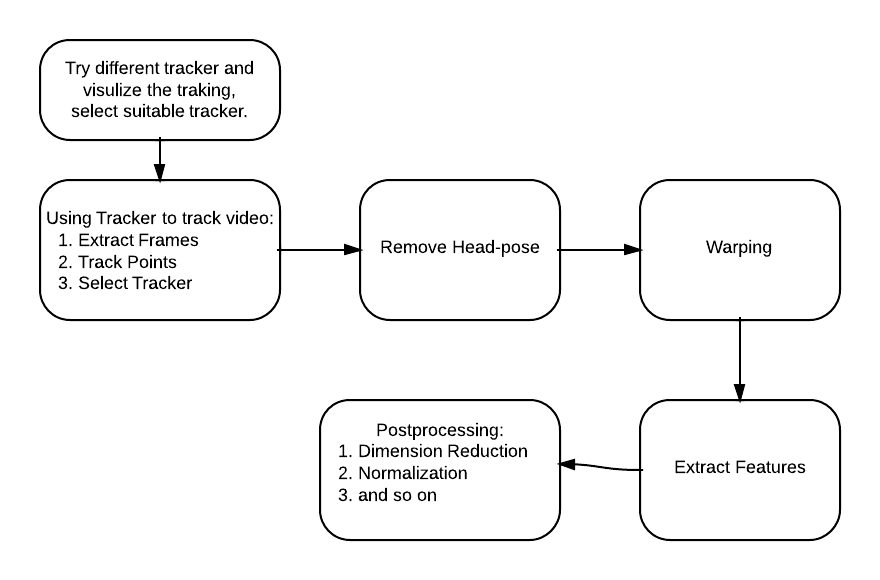
\includegraphics[width=\textwidth]{imgs/ProcedureChart.png}
\caption{Main Procedure}
\label{fig:proc}
\end{figure}
Figure \ref{fig:proc} shows main procedure of the whole project. At beginning, I tried several trackers. Intraface and DRMF are two trackers I tried and compared most. Two trackers are using different methods and also implemented in different languages. Intraface are programmed in c and matlab and has great interface for matlab. I tried two version of DRMF, DRMF programmed using CUDA which uses parallel processing is quite fast. As the programme of DRMF doesn't integrate extract frames from videos. The images are extracted using external function, then tracked using DRMF. I choose Intraface as the final choose, the reason and comparison will be given in later section. Remove head-pose seems to be a very important part for this project, as subject's head moves frequently in many videos. After having tracking points without head-pose, each face in each frame is warped and scaled to same size grey image. Extracting features is to extract appearance feature of each face in the image. Post-processing is preprocessing before using the data for classification.
\paragraph{Data flow Chart}
\begin{figure}[ht]
\centering
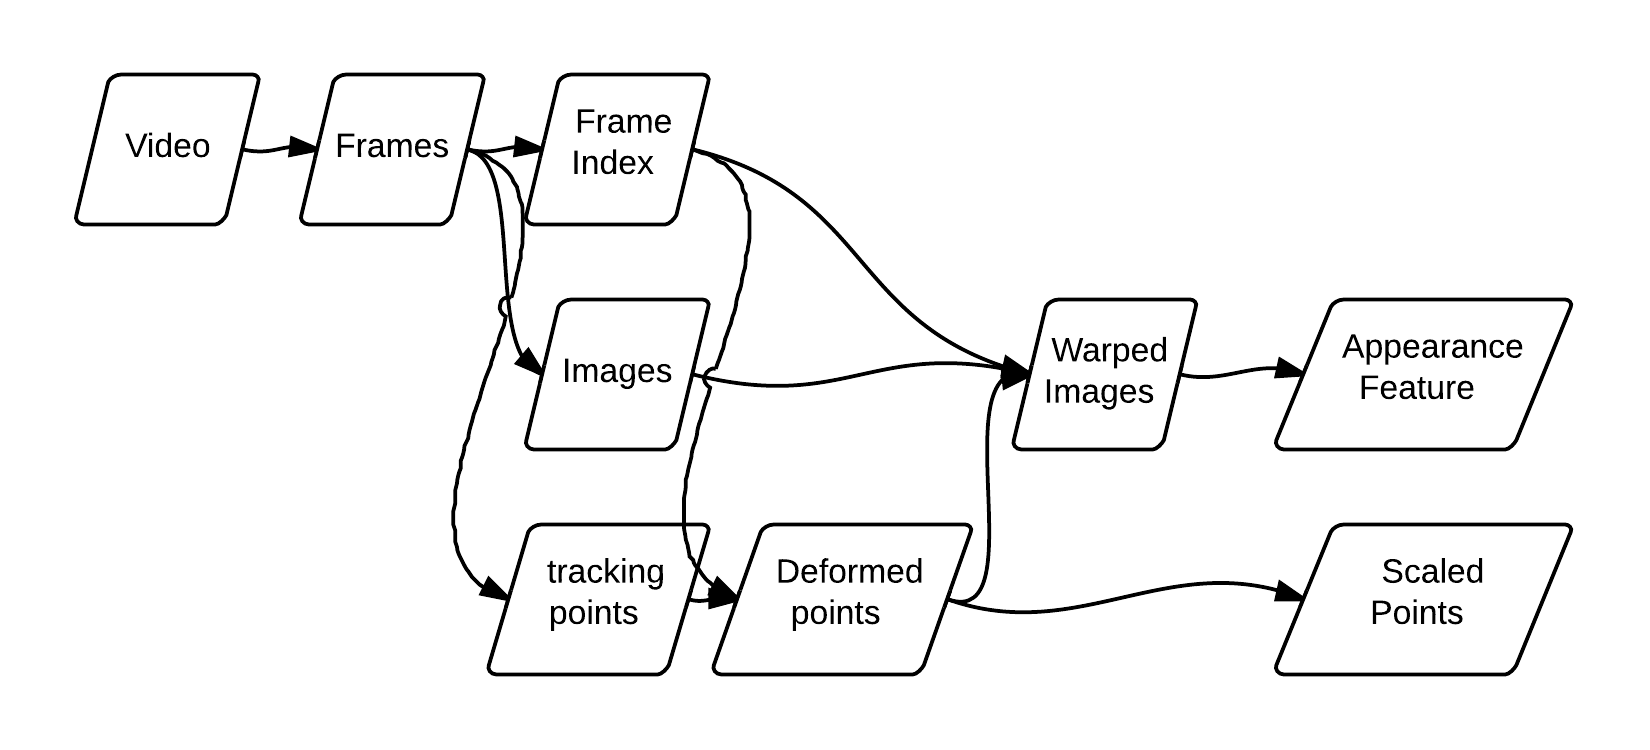
\includegraphics[width=\textwidth]{imgs/DataFlowChart.png}
\caption{Data Flow}
\label{fig:DF}
\end{figure}
Figure \ref{fig:DF} show data I need for processing. There are two types of encoded video, one is in format of fly and the other is avi. Extracting frames from videos is proceed with Intraface and stored in formats of jpeg and mat which used for processing of matlab. There are several situations that a track is unable to track a face in the image such as no subject in the image, the head is face to a very large angle from frontal face, face is partially not show in the frame. Frame index points to those images which the tracker is able to tracker a face in a frame. Image is the frame images stored in mat format. Different tracker may tracks different number of characteristic facial points. Intraface tracks 49 facial points and DRMF tracks 66 points. Deformed points is the tracking point after removed head-pose. Warped Images is the face after remove head-pose and background which only leaves the meshes build by tracking points. Appearance feature is face feature extracted using local binary pattern (LBP). As the image size from image to warped images are changed, the points is rescaled from deformed point to scaled points.

\section{Face Alignment}

Face alignment is to align face in one image with respect to the same face in another image. Face alignment techniques are used to track characteristic facial points in image sequences. In this project, the aim of face alignment is to localise the feature points on face images. The points are usually around eyes, nose, mouth, and outline. Face alignment techniques are essential on face recognition, modelling and synthesis. There are three main different approaches Parametrized Appearance Models(PAMs), Discriminative approaches, Part-based deformable models. Parametrized appearance models contains many models such as active appearance models (AAMs), morphrable models, eigentrackings, and template tracking \cite{xiong2013supervised}. All these models are using Principle Component Analysis(PCA) method to parametrize a face. A face could approximately decomposed as linear combination of shape basis and appearance basis. The problem of face alignment could be refer as minimising the difference between the constructed PAM and the face. Common approach is use Gauss-Newton methods \cite{xiong2013supervised}. Discriminative approaches are to learn the linear regression between the head move and appearance change. Part-based deformable model perform face alignment by maximising the posterior likelihood of part locations given image\cite{xiong2013supervised}.

\subsection{Active Appearance Model}
Active Appearance Model (AAMs) is defined as a generative model of a certain visual phenomenon in \cite{matthews2004active}. AAMs are conceptually related to morphable models, constrained models and active blobs. In this project, it is refer to a model of face. As AAM is conceptually related to other parameterized appearance model, so it is introduced as an example of parameterized appearance model for understanding purpose. According to \cite{matthews2004active}, there are two types of AAMs, one refers as independent shape and appearance models, which model shape and appearance independently, and the other refers as combined shape and appearance models, which parameterized shape and appearance model with a single set of linear parameters \cite{matthews2004active}. Normally AAMs appears along with a fitting algorithm. However, in the following context, it only refers to a model.\cite{matthews2004active} gave a well explain about what is an AAM, most of following theory are from \cite{matthews2004active}.
\paragraph{Shape}
Shape of a face $s$ is defined by coordinates $(x,y)$ of $v$ vertices of face points and the mesh they built:
\begin{equation}
s = (x_{1},y_{1},x_{2},y_{2},...,x_{v},y_{v})^{T}
\end{equation}
\newline
$s$ also can be expressed as a base shape $s_{0}$ plus linear combination of $n$ shape vectors $s_{i}$:
\begin{equation}
s = s_{i} + \sum_{i =1}^{n}p_{i}s_{i}
\end{equation}
\paragraph{Appearance}
For all pixels x in the mesh $s_{0}$, appearance $A(0)$ can be expressed by base appearance $A_{0}(x)$ and m appearance images $A_{i}(x)$.
\begin{equation}
A(x) = A_{0}(x) + \sum_{i=1}^{m}\lambda_{i}A_{i}(x) \qquad \forall x \in s_{0}
\end{equation}
\newline
AAMs are usually computed by applying Principle Component Analysis (PCA) to choose images. The chosen images contains a variety of shapes. The base shape $s_{0}$ is the mean shape and the vector $s_{v}$ is the eigenvector corresponding to the largest $v$ eigenvalues. The base appearance $A_{0}$ and the appearance $A_{i}$ is computed by applying Principle Component Analysis to a set of shape normalised images.
\paragraph{Model} 
$W(x:p)$ is the warp from $s_{0}$ to $s$. Then the model $M$ set the appearance of $W(x:p)$ to $A(x)$.
\begin{equation}
M(W(x:p)) = A(x)
\end{equation}
\newline
Combined AAMs
\newline
Combined AAMs just use parameter $c = (c_{1},c_{2},...)^{T}$ to parametrize shape:
\begin{equation}
s = s_{0} + \sum_{i=1}^{l}c_{i}s_{i}
\end{equation}
and appearance:
\begin{equation}
A(x) = A_{0}(x) + \sum_{i=1}^{l}c_{i}A_{i}(x)
\end{equation}
\begin{figure}[ht]
\centering
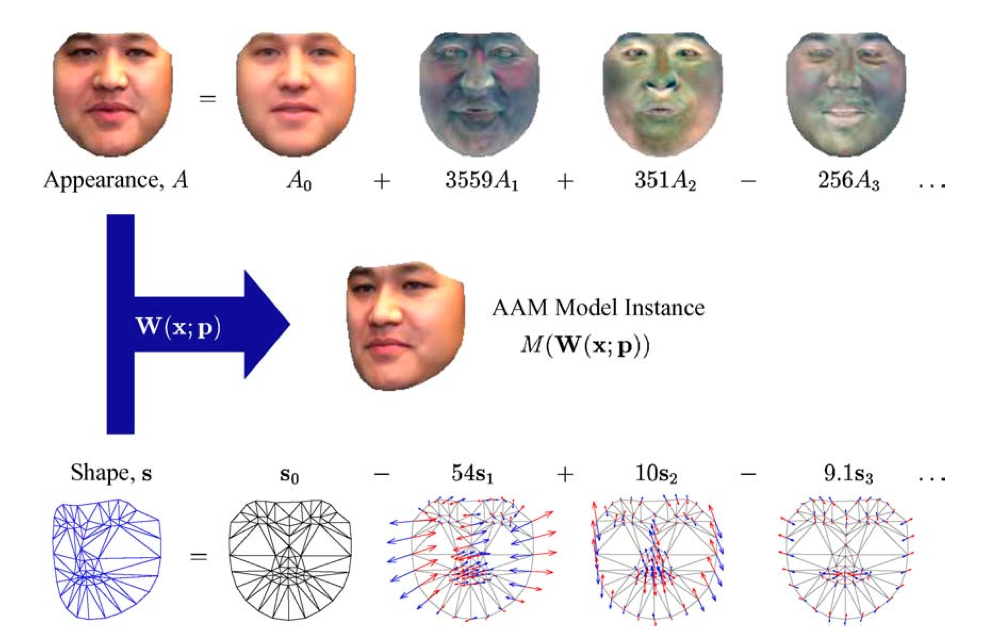
\includegraphics[width = \textwidth]{imgs/AAM_Model.png}
\caption{An AAM instantiation from \cite{matthews2004active}}
\label{fig:AAMI}
\end{figure}
An example of AAM instantiation is clearly shown in figure \ref{fig:AAMI}.
\subsection{Trackers}
There are many different trackers for tracking facial feature points. Different tracker may using different approaches, so they are suitable for different situations. I tried two main trackers for tracking characteristic facial points, one is Intraface \cite{xiong2013supervised} which use suppervised decent method, the other is DRMF \cite{asthana2013robust} which use discriminative response map fitting. According to my using experiment, Intraface is very good at tracking motion face and DRMF is very good at fitting face model to a more standard face even with low resolutions. The number of facial points they track are also differnt.
\subsubsection{Intraface}
\cite{xiong2013supervised} implies image alignment  can be posed as solving a nonlinear optimization problem. It uses Supervised Descent Method for minimising Non-linear Least Square(NLS) function, which avoids calculating the Hessian and the Jacobian that could be computationally expensive. For this reason, the running time of Intraface shows that the method is very effective and efficient.
\paragraph{Tracking Points}
Figure \ref{fig:IPI} shows the tracking points of Intraface. This tracker tracks 49 facial feature points. As you can see the eyes, nose, mouth, unfortunately the jaw and cheek may contain visual information that may help classification.
\begin{figure}[ht]
\centering
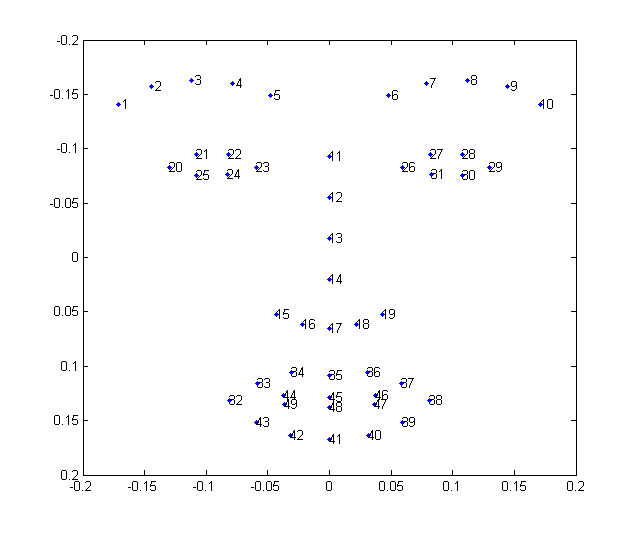
\includegraphics[width = 80mm]{imgs/FacialIndexIntraface.png}
\caption{Intraface landmark points}
\label{fig:IPI}
\end{figure}
\paragraph{Eating and Talking Sequence}
Figure \ref{fig:IES} shows a sequence of image of eating tracked by Intraface. The point are aligned very precisely along the face. Figure \ref{fig:ITS} shows a talking sequences of image tracked by Intraface. The landmark points of mouth is very accurate.
\newpage
\begin{figure}[p]
\centering
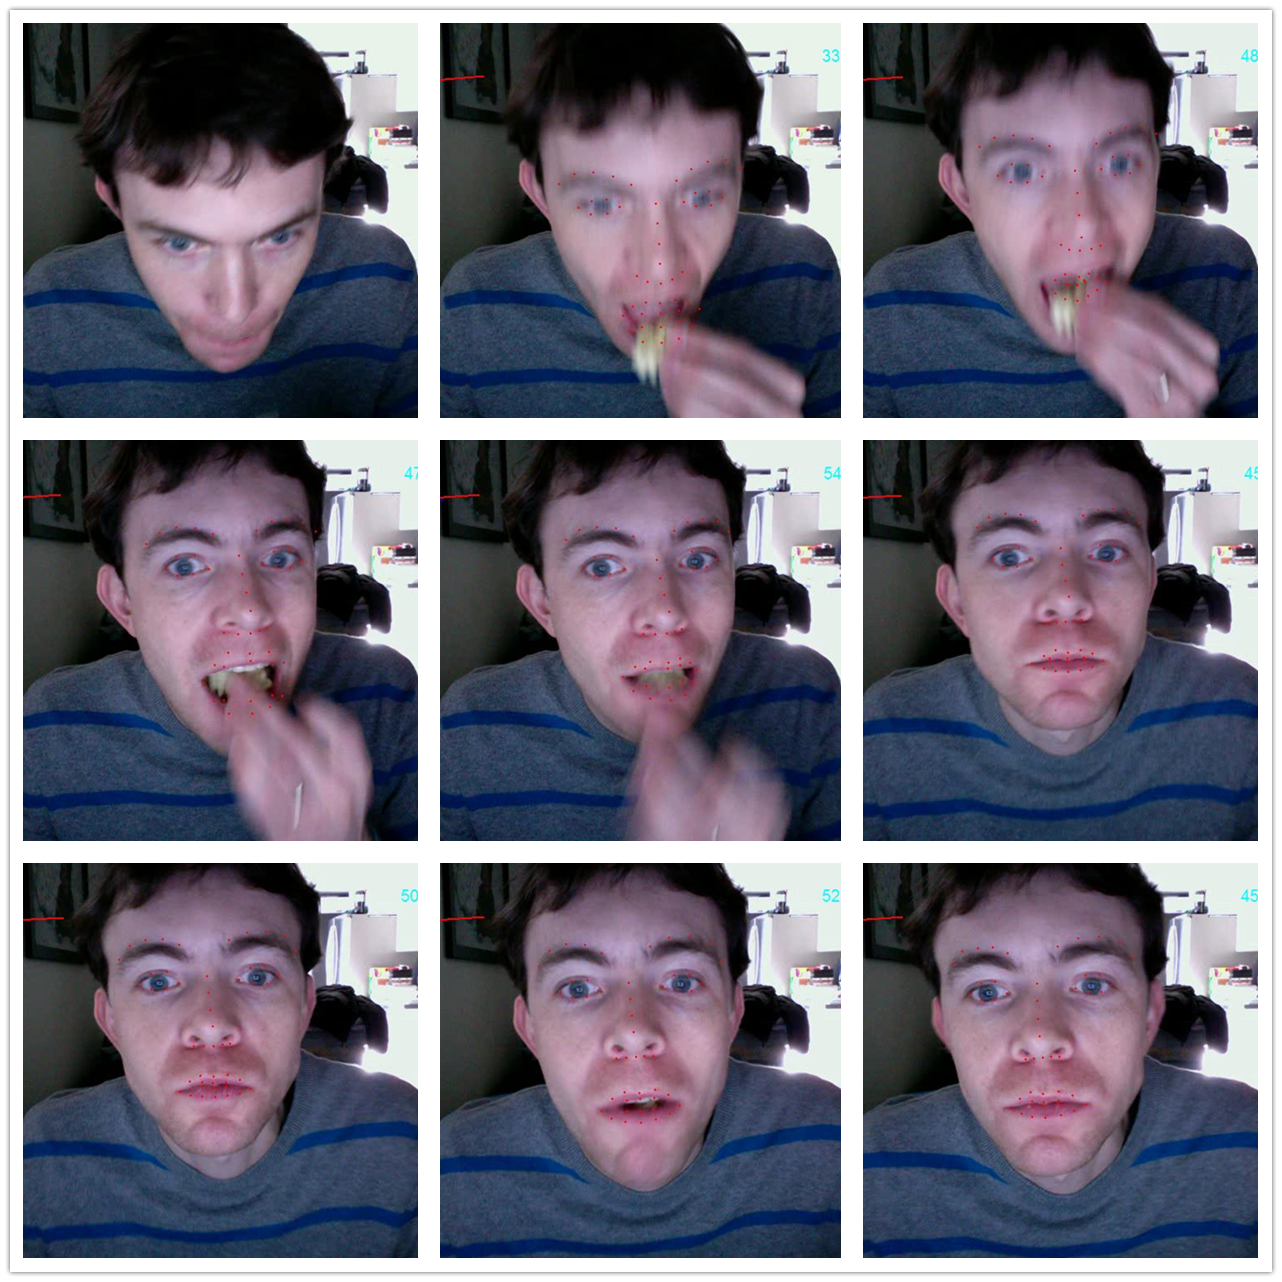
\includegraphics[width=110mm]{imgs/Tracking_Intraface_eating_red.png}
\caption{Eating sequence tracked by Intraface}
\label{fig:IES}
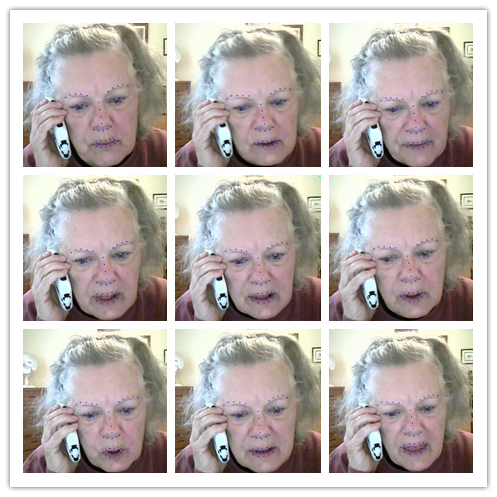
\includegraphics[width=110mm]{imgs/Talking_Intraface_140711_176_184.png}
\caption{Talking sequence tracked by Intraface}
\label{fig:ITS}
\end{figure}
\newpage
\subsubsection{DRMF}
DRMF uses novel discriminative regression based on Constrained Local Models(CLMs) for face alignment\cite{asthana2013robust}. The basic idea of DRMF is to fit a face for each frame of a video. After locating the position of a face, the tracker tries to fit a trained constrained local model to fit the face. Sometimes the fitting result is not very good and the landmark points of mouth region is not very accurate.
\paragraph{Tracking Points}
Figure \ref{fig:DPI} shows 66 facial feature points tracked by DRMF, the extra 17 points are the point around face bound. Other landmark points are at the same order as Intraface.
\begin{figure}[ht]
\centering
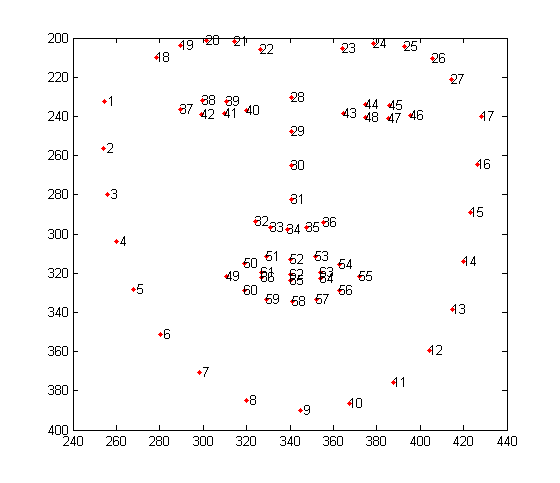
\includegraphics[width = 80mm]{imgs/FacialIndexDRMF.png}
\caption{DRMF landmark points}
\label{fig:DPI}
\end{figure}
\paragraph{Talking and Talking Sequence}
Figure \ref{fig:DES} and \ref{fig:DTS} show image sequences of eating and talking tracked by DRMF. It is easy to see that the facial feature points are not aligned as better as Intraface. However, the advantage of DRMF is that with the extract bound points of face, we are able to extract the visual information about the jaw and cheek, which may be helpful for classification.
\newpage
\begin{figure}[p]
\centering
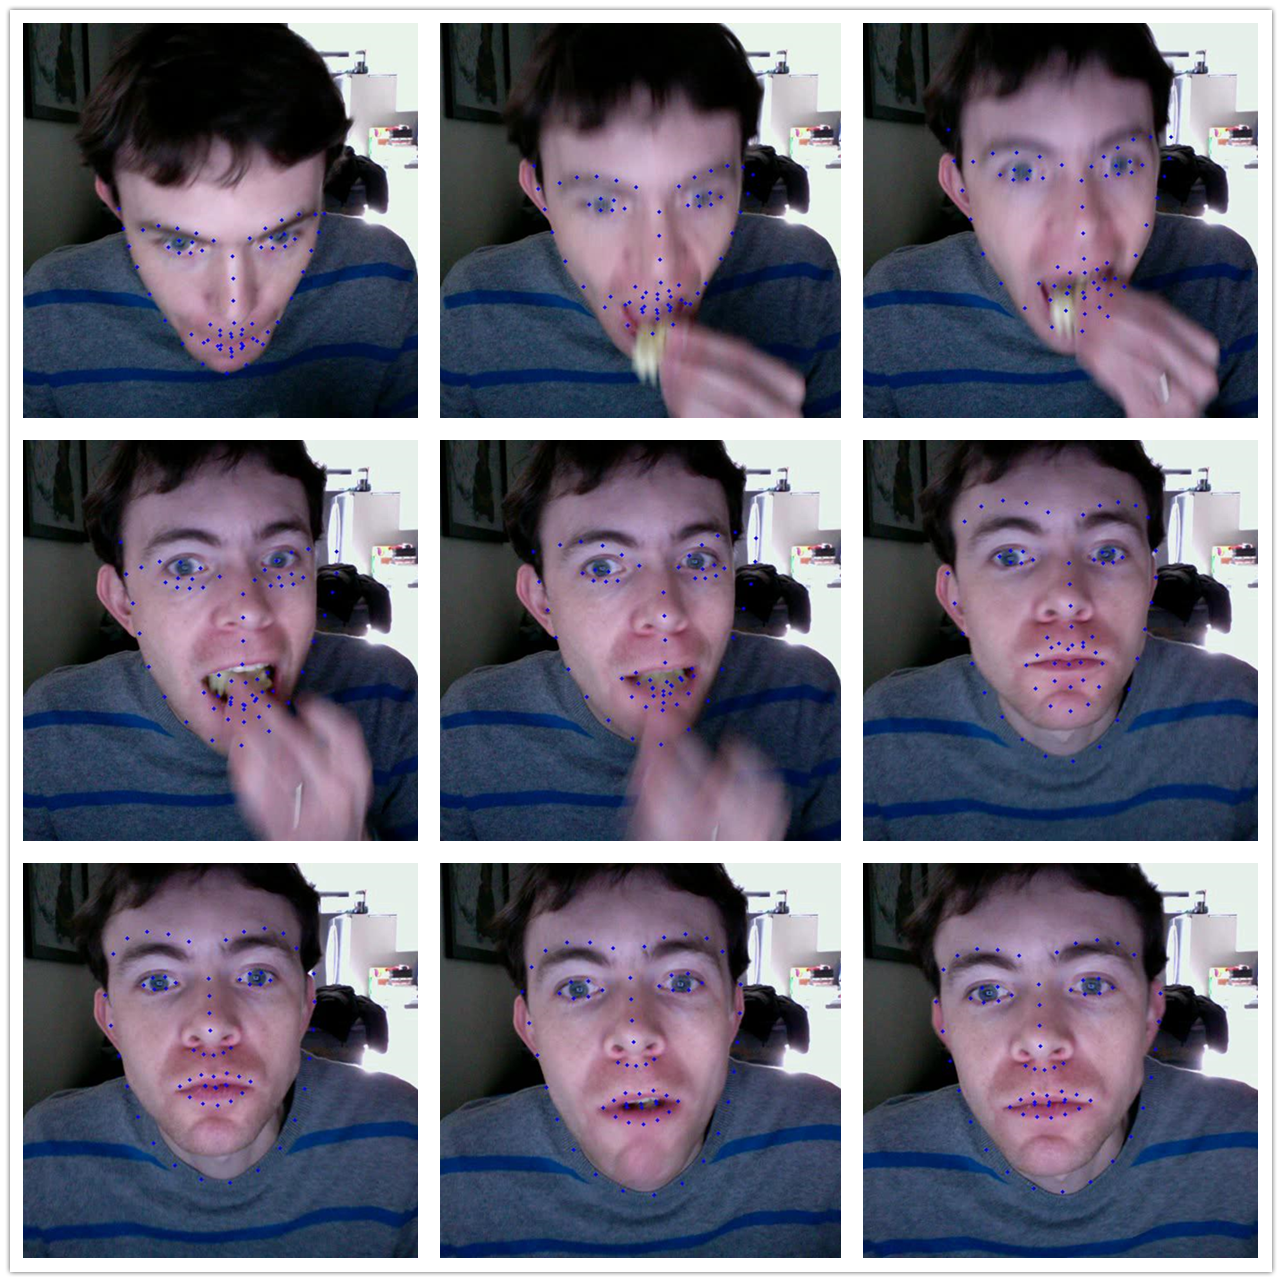
\includegraphics[width=100mm]{imgs/Tracking_DRMF_eating.png}
\caption{Eating sequence tracked by DRMF}
\label{fig:DES}
\includegraphics[width=100mm]{imgs/Talking_DRMF_140711_176_184.png}
\caption{Talking sequence tracked by DRMF}
\label{fig:DTS}
\end{figure}
\newpage
\subsection{Comparison}
The following are some examples for comparing two trackers. Intraface is generally better than DRMF in accuracy and efficient. There are two version of DRMF tracker one is implemented by CUDA language the other is by C language. Although the C version of DRMF is very slow and very easy to run out of memory, the version implementd by CUDA is very fast as CUDA is using parallel computing. However, for face points alignment, DRMF is not as accurate as Intraface. In some situations, DRMF try to fit a face and the fitting result is awful. The images with red points are tracked by Intraface, and the images with blue points is tracked by DRMF.

In figure \ref{fig:cmp01}, compare top left and top right images, we can see Intraface does not track the face of the smaller face, DRMF tracked the smaller face instead of the large face. This shows the advantage of DRMF on track face of low resolution face. I tried to use Intraface to track a image with multiple face, Intraface is able to track multiply faces in one image. So this means, Intraface is not good at tracking face on low resolution face. Compare the lower two images on the right hand side, the feature points of nose is not proper aligned, this is caused by imperfect of the fitting algorithm. The feature points of face bound are also not well aligned. Comparing the alignment of eye alignment on the left hand side of both tracker, Intraface is better than DRMF. The feature points of right eye brows of the mid right image are also not algined precisely.

In figure \ref{fig:cmp02}, in the top left image, DRMF is unable to fit a face to the face as the face is facing to the left. Of course, Intraface is unable to apply face alignment to a image doesn't show half of the face like this, it choose to ignore this image. In lower two images on the left hand side shows two situations that DRMF fail to fitting face model to face because of the face is partial out of the image frame. The middle one shows that the fitting face points are force to stay in the frame and the mouth are moved up to close nose. The lower one image shows that as most of mouth region is out of frame, the model is fitted to the left eye forcefully. The middle and lower images on the right hand side shows that Intraface would ignore those points that are out of frame. It seems using Supervised Descent Method is very good at tracking face that moves. However, there is a bug of this tracker, while tracking the video, if the subject moves hand to cover the mouth, the points of mouth would be pushed upwards, and it will not come back even the hand is moved away, unless, the tracker loss the face and re-track the face.
\begin{figure}
\centering
\includegraphics[width=110mm]{imgs/Tracking_Intraface_DRMF_compare_00.png}
\caption{Tracking result: images with red points on the left hand side are tracked by Intraface and images with blue points on the right hand side are tracked by DRMF}
\label{fig:cmp01}
\includegraphics[width=110mm]{imgs/Tracking_Intraface_DRMF_comparison.png}
\caption{Tracking result, images with red points on the right hand side are tracked by Intraface and images with blue points on the left hand side are tracked by DRMF}
\label{fig:cmp02}
\end{figure}
\newpage
\section{Remove Head-pose}
Subjects were unrestricted while they were recording the video, their head pose are vary different. The coordinate of facial feature points are different for each video frame. In order to unite the head, we need to remove the head pose from the coordinates of facial feature points.  If define the horizontal direction is x, the vertical direction is y and z is the direction, subject facing camera. It is very easy to remove head-pose in x-y direction, just by rotating and scaling the points would remove the head-pose. If the subject had a head-pose in x-z and y-z direction, it would be hard to find the correct transformation matrix for tracked facial points. The algroithm of removing head-pose from tracking points is \cite{saragih2011deformable}. Basically, it has a deformable 3-D Constrained Local Model(CLM), minimize the error of fitting the model and the 2D points and then remove head-pose and give the new 2D points. Figure \ref{fig:RHP} gave two example of orginal track points and deformed points. From figure \ref{fig:RHP}, we can see this method could remove head-pose without losing information of mouth shape.
\begin{figure}[ht]
\centering
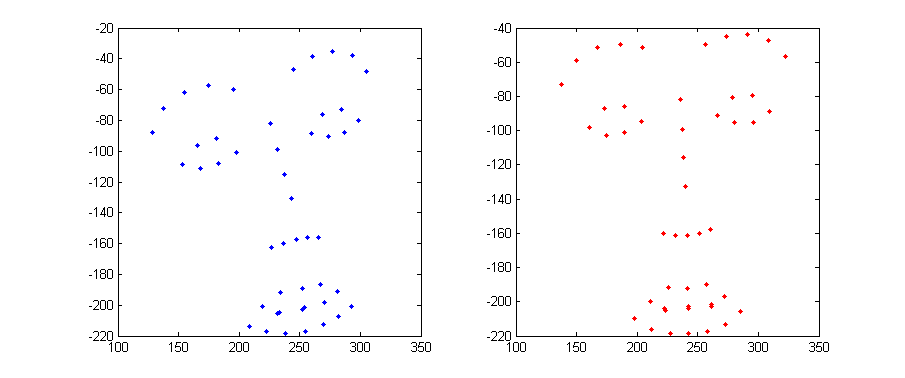
\includegraphics[width=.6\textwidth]{imgs/160954_Deform_233.png}
\caption{Traking points and Deformed Points Example}
\label{fig:RHP}
\end{figure}
\section{Warping}
There are two types of features we need to extract, shape feature and appearance feature, the previous section just remove heap-pose of shape feature vector. The appearance of face on image is not correctly showing a face that could be directly used for classification, as the face is not facing to frontal. In order to have head-pose free face, we need to distort the image to the one we need. In here I use Piece-wise Affine\cite{AAMWarp} to warp the image. According to the model in Active Appearance Model. We need to warping image from one to another with respect to the mapping of shape feature points set ${p_{1},p_{2},...p_{n}}$ into another point set ${p'_{1},p'_{2},...p'_{n}}$. Each point is represented as $p = [x,y]^{T}$. The mapping function would be:
\begin{equation}
f(p_{i}) = p'_{i} \quad \forall \ i = 1...n
\label{eq:W1}
\end{equation}
\newline
Piece-wise Affine assume that f is locally linear. In 2-D framework like 2-D AAM, first find the mesh-grid constructed by all shape feature points. Delaunay triangulation is a good way to express it. In Delaunay triangulation, there is no points inside its circumcise. Then the problem is to find the mapping function $f$ to map the triangle mesh of the first point set and the second point set. For each points on each triangle of the first point set $I$ can be mapped to unique points on each triangles of the second point set $I'$ by affine transformation, which is combination of translation, rotation and scaling. Assume $p_{1}$, $p_{2}$ and $p_{3}$ are a vertices of a triangle in $I$, then the points inside the triangle can be written as:
\begin{equation}
\begin{split}
p 
& = p_{1} + \beta (p_{2}-p_{1})+\gamma (p_{3}-p_{1}) \\
& = (1-\beta-\gamma)p_{1} + \beta p_{2} + \gamma p_{3} \quad \quad assume \: \alpha + \beta + \gamma = 1\\
&  = \alpha p_{1} + \beta p_{2} + \gamma p_{3}
\end{split}
\end{equation}
\newline
As points $p$ are in the triangle, so $\alpha\geq 0$,$\beta,\gamma \leq 1$. Then the corresponding points $p'$ in image $I'$ inside corresponding triangle would also satisfy the equation:
\begin{equation}
p' = f(p) = \alpha p'_{1} + \beta p'_{2} + \gamma p'_{3}
\label{eq:FX}
\end{equation}
We have the three points of a triangle, it is easy to determine the value of $\alpha$,$\beta$ and $\gamma$ by solving two linear equation for a know points, $p = [x,y]^{T}$:
\begin{equation}
\label{eq:CABR}
\begin{split}
\alpha & = 1 - (\beta + \gamma) \\
\beta  & = \frac{yx_{3}-x_{1}y-x_{3}y_{1}-y_{3}x+x_{1}y_{3}+xy_{1}}{-x_{2}y_{3}+x_{2}y_{1}+x_{1}y_{3}+x_{3}y_{2}-x_{3}y_{1}-x_{1}y_{2}} \\
\gamma & = \frac{yx_{2}-xy_{1}-x_{1}y_{2}-x_{2}y+x_{2}y_{1}+x_{1}y}{-x_{2}y_{3}+x_{2}y_{1}+x_{1}y_{3}+x_{3}y_{2}-x_{3}y_{1}-x_{1}y_{2}}
\end{split}
\end{equation}
\newline
Equation \ref{eq:CABR} give the function to calculate $\alpha$,$\beta$,$\gamma$, with the Equation \ref{eq:FX}, we can calculate all the points in image $I'$. Peudo-code of piece-wise affine warp would be:
\begin{enumerate}
\item For each point $p = [x,y]^{T}$ inside image $I$
\item Determine which triangle $p$ is in
\item Use equation \ref{eq:CABR} to calculate $\alpha$,$\beta$,$\gamma$
\item Use equation \ref{eq:FX} to calculate the corresponding position of $p'$
\item set the value of $p'$ in $I$ to the value of $p$ in $I$
\item end
\end{enumerate}
The follow is the warping result, the image was not highly distorted as the face is basically facing to the frontal. However, it is easy to notice the face is a little rotated to the right and there is a small change on the shape of mouth.
\begin{figure}[ht]
\centering
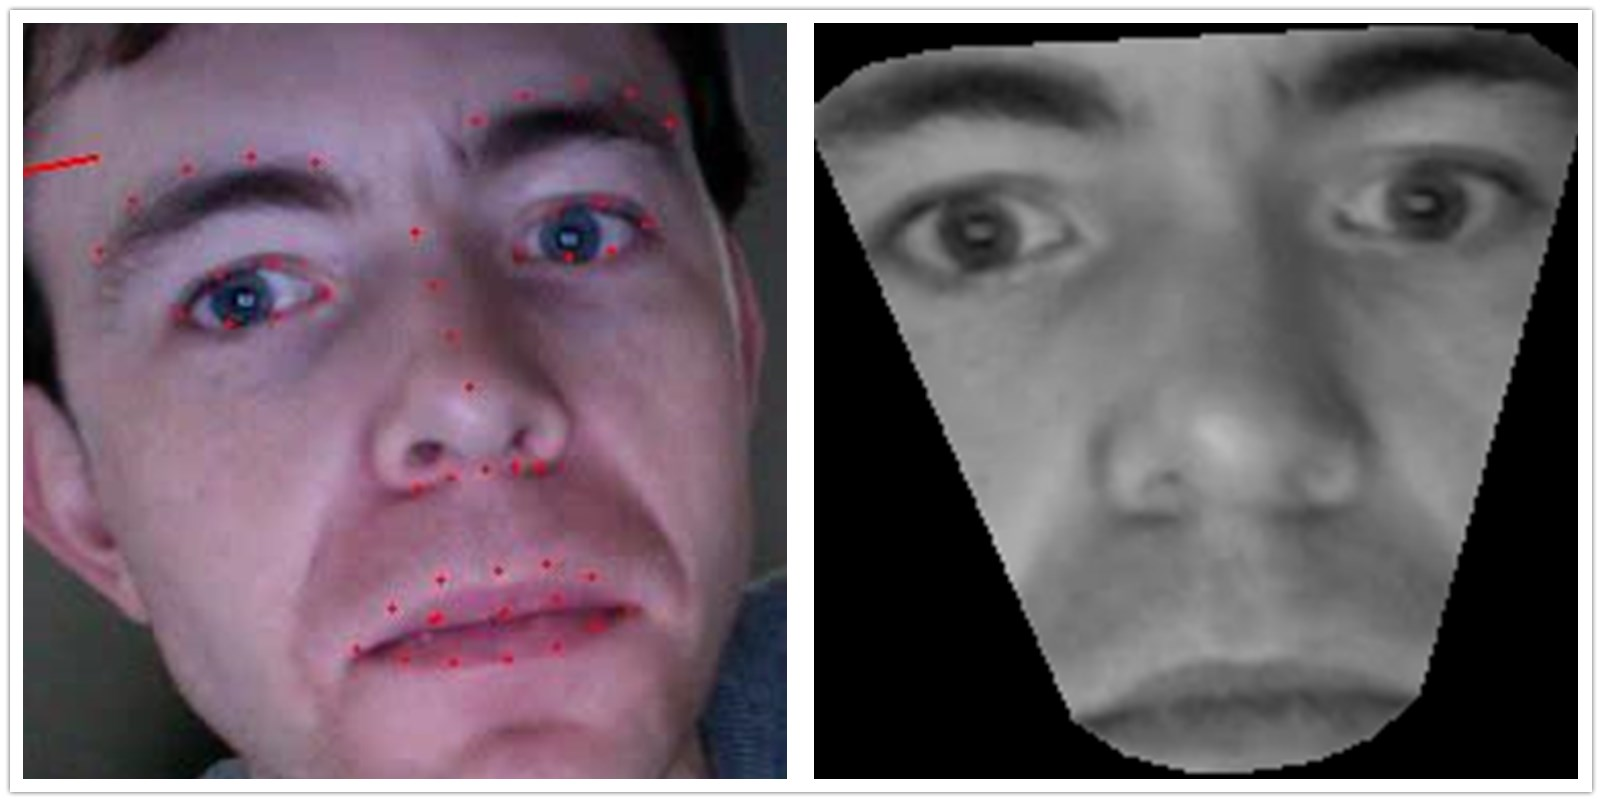
\includegraphics[width=.5\textwidth]{imgs/Warping_Intraface_213.png}
\caption{Talking sequence tracked by Intraface}
\end{figure}
\section{Feature Extraction}
The warped images are not directly used for classification, as the image value are sensitive to illumination, and noise. In addition, the dimensionality of image vector could be very large. An effective facial representation from original image is vital for classification. Experiments of \cite{shan2009facial} shows that Local Binary Pattern(LBP) features are effective and efficient for facial expression recognition. The best performance of \cite{shan2009facial} is obtained by combing Support Vector Machine and Boosted-LBP features. \cite{shan2009facial} also shows that LBP feature perform stably and robustly on low-resolution facial expression recognition. There are several reasons to use LBP: firstly LBP is robust to monotonic changes in illumination shown in figure \ref{fig:LBPE00}; secondly, computational simplicity, the calculation only contain integer math and there is no need for preprocessing; thirdly, the time complex is $O(n)$.
\begin{figure}[ht]
\centering
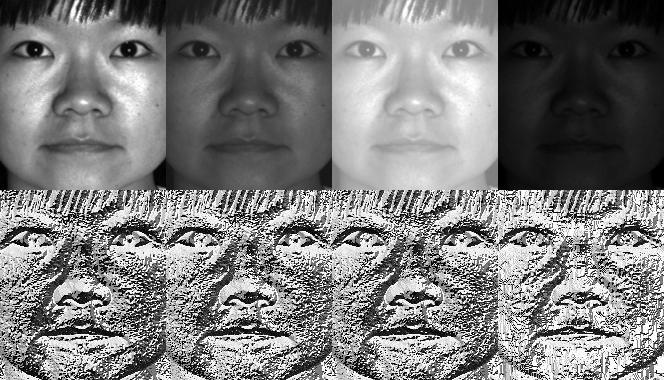
\includegraphics[width = .5\textwidth]{imgs/lbp_yale.jpg}
\caption[The LOF caption]{LBP Example\footnotemark}
\label{fig:LBPE00}
\end{figure}
\footnotetext{LBP Example From \url{http://docs.opencv.org/modules/contrib/doc/facerec/facerec_tutorial.html#id22}}
\subsection{Local Binary Pattern}
Texture is an important characteristic of images and videos. 2-D surface can be characterized by two properties: pattern and contrast. In the warping step, the image was transformed to gray scale and we need a grayscale rotation invariant pattern to measure. LBP is invariant to any monotonic gray level change and it is easy to compute. Ojala et al(1996) introduced the fist generation of LBP operator \cite{shan2009facial}, it was proved to be a powerful texture descriptor. Figure \ref{fig:LBPE01} show how to calculate LBP value of a pixel and the contrast of the pixel.
\begin{figure}[ht]
\centering
\captionsetup{justification=centering,margin=3cm}
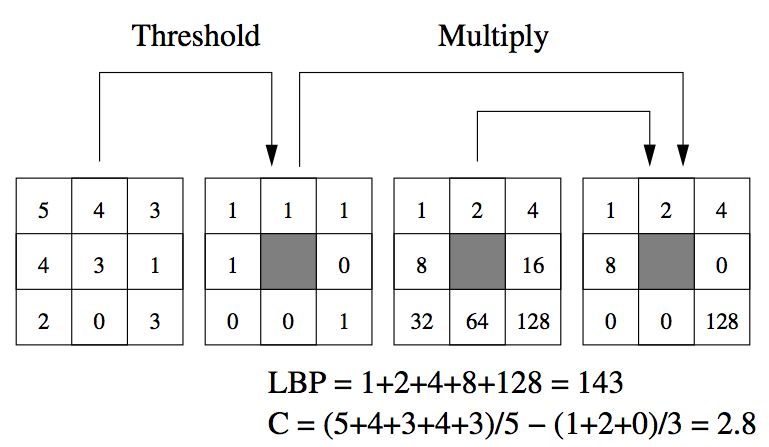
\includegraphics[width = .6\textwidth]{imgs/LBP_Example_1.png}
\caption{An Example of Calculating LBP code and \newline a contrast measure of single pixel, image from \cite{maenpaa2005texture}}
\label{fig:LBPE01}
\end{figure}
\newline
The binary number could be used for coding types of curved edges, spots, flat area, etc as shown in figure \ref{fig:LBPE02}. Figure \ref{fig:LBPE02} is using circular pattern. In implementation, the on-grid points($g_{0}-g_{4}$points in figure \ref{fig:LBPE03}) directly use sample data for calculation, but the off-grid points(the points in the second grid($P=8,R=1$), not in grid($P=4,R=1)$) in figure \ref{fig:LBPE03}) are calculating using interpolation. The 3X3 structure can not capture dominant feature for large scale structure\cite{shan2009facial}. So Ojala et al extend LBP to multiple scales as shown in figure \ref{fig:LBPE03}.
\begin{figure}[ht]
\centering
\captionsetup{justification=centering,margin=3cm}
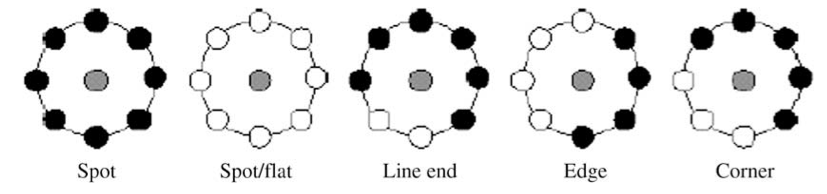
\includegraphics[width = .6\textwidth]{imgs/LBP_Example_2.png}
\caption{An Example of feature type coded by LBP and \newline black circles present ones and white circle represent zeros, image from \cite{shan2009facial}}
\label{fig:LBPE02}
\end{figure}
\newline
Define the operator as $LBP_{P\ R}$. Define texture T in local neighbourhood as the joint distribution of gray level of P image pixels, R is the spatial resolution to the central pixel.
\begin{equation}
T = t(g_{c},g_{0},...g_{P-1})
\label{eq:LBPDT}
\end{equation}
\begin{figure}[ht]
\centering
\captionsetup{justification=centering,margin=1cm}
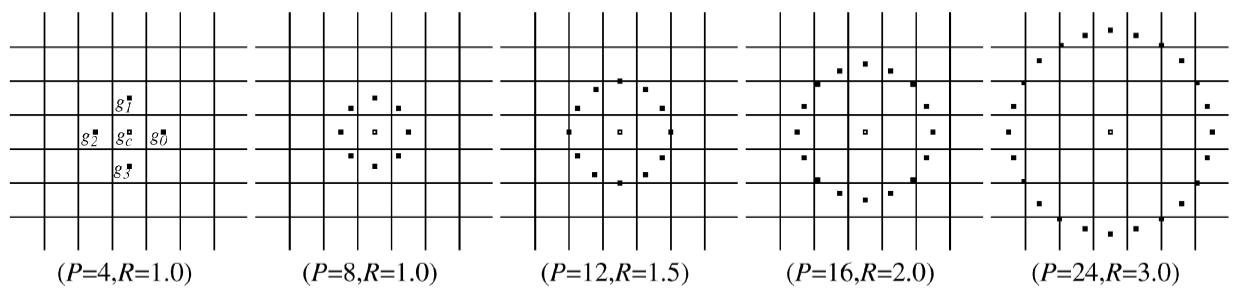
\includegraphics[width = \textwidth]{imgs/LBP_Example_3.png}
\caption{An example for multiscale circular pattern, image from \cite{ojala2002multiresolution}}
\label{fig:LBPE03}
\end{figure}

Ojala et al proposed multi-scale LBP in \cite{ojala2002multiresolution}, which could be used for arbitrary circular neighbourhoods and multiple scales; extend operator, uniform patterns, which can help reduce the feature vector. Uniform Local Binary Pattern is defined as patterns with at most two contiguous regions. The uniform pattern is as shown in figure \ref{fig:LBPE04}. Uniform Patter have significant effect on dimension reduction as the 256($2^8$) elements can be reduced to 59 elements, with 7*8 (uniform pattern from 1-7 in figure \ref{fig:LBPE04}, as there are 8 directions) + 2 (uniform pattern 0 and 8)+ 1 (represent non-uniform patterns). In addition, most natural images are uniform LBP and uniform pattern is more robust than non-uniform pattern that it perform better result in many applications.
\begin{figure}[ht]
\centering
\captionsetup{justification=centering,margin=1cm}
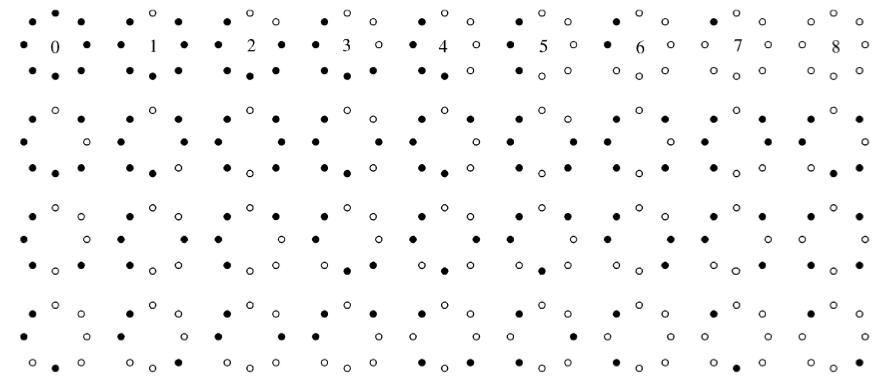
\includegraphics[width = \textwidth]{imgs/LBP_Example_4.png}
\caption{The first row are nine uniform patterns, Black represent 1, white represent 2, image from \cite{ojala2002multiresolution}}
\label{fig:LBPE04}
\end{figure}
\newpage
\section{Postprocessing}
As it is known large margin classifiers are sensitive to the way features are scaled, it's better to normalize either the data or the kernel function \cite{ben2010user}. Feature of a image is represented by a vector, the number in the vector would influence the weight of feature in this dimension. As I would like to treat each dimension similar, I scale the number in the range of $[0,1]$.
\paragraph{Normalization}
The performance of SVM is usually better if the data is normalized. There are two ways of applying normalization, standardizing the input features or normalizing the kernel function. As I am using the built-in function of libsvm \cite{CC01a}, so I standardising the input features by subtracting its mean and divide by its standard deviation.
\paragraph{Scaling}
The range of appearance feature vector and shape feature vector is different. I would like to treat then as the same. So I scale all the vector into the range of $[0, 1]$, by subtract the minimum and divide by the maximum number of each dimension.